\chapter{NIO} 

	本章将对"New I/O"工具包的主要应用进行介绍。NIO主要包括两个部分:

	java.nio.channels包介绍了Selector和Channel抽象,java.nio包介绍了Buffer抽象。这都是一些高级的特性,有许多微妙的使用细节,因此,本章的组织结构也与前面的章节略有不同。第1节通过介绍它们所要解决的具体问题来引出NIO特性--尤其是当没有这些特性时,构建高性能服务器所面临的挑战。(如果你并不关心"为什么?"这类问题,可以直接跳过本节。)在第5.2节,我们将像前面一样展示一个(TCP)"回显"协议客户端,以介绍SocketChannel和Buffer类的使用方法,以及Channel非阻塞特性(nonblocking),这与第4.2节中介绍的阻塞特性有所不同。第5.3节中展示了一个使用了Selector,Channel和Buffer抽象服务器。

	然后我们回到主要抽象数据类型的使用细节上,各自用一小节进行介绍。最后,在第5.7节介绍了DatagramChannel类(DatagramSocket类的信道化版本)。 

\section{为什么需要NIO} 

	基本的Java套接字对于小规模系统可以很好地运行,但当涉及到要同时处理上千个客户端的服务器时,可能就会产生一些问题。其实在第4章已经可以看到一些迹象:由于创建、维护和切换线程需要的系统开销,一客户一线程方式在系统扩展性方面受到了限制。使用线程池可以节省那种系统开销,同时允许实现者利用并行硬件的优势。但对于连接生存期比较长的协议来说,线程池的大小仍然限制了系统可以同时处理的客户端数量。考虑一个在客户端之间传递消息的即时消息服务器(Instant Messaging)。客户端必须不停地连接服务器以接收即时消息,因此线程池的大小限制了系统可以同时服务的客户端总数。如果增加线程池的大小,将带来更多的线程处理开销,而不能提升系统的性能,因为在大部分的时间里客户端是处于闲置状态的。 

	如果这就是所有问题,可能NIO还不是必要的。不幸的是,在使用线程的扩展性方面还涉及一些更加难以把握的挑战。其中一个挑战就是程序员几乎不能对什么时候哪个线程将获得服务进行控制。你可以设置一个线程实例的优先级(priority)(高优先级的线程相对于低优先级的线程有优先权),但是这个优先级只是一种"建议"--下一个选择执行的线程完全取决于具体实现。因此,如果程序员想要保证某些连接优先获得服务,或想要指定一定的服务顺序,线程可能就很难做到。

	然而,有关线程的最重要的问题可能是我们至今还未提及。那是因为在"回显服务"示例程序中,每个客户端都与其他客户端相互独立,客户端之间没有交互,也不会影响服务器的状态。但是在实际情况中,大多数的服务器有一些信息(称为"状态")需要由不同的客户端同时访问或修改。例如,考虑一种允许大城市的市民保留一个小时停车位的服务。计划什么时间段由谁获得哪个停车位必须保持一致,而且,该服务必须保证同一用户在同一时间段内最多只能获得一个停车位。这些限制就要求在所有客户之间共享一些状态信息(即调度表)。这需要通过使用锁(locks)机制或其他互斥机制对依次访问状态进行严格的同步(synchronized)。否则,由于调度程序能够使不同线程上的程序段在一定程度上交错执行,如果不同线程试图同时更新调度表,它们就可能改写掉其他线程所作的修改。 

	由于需要对共享状态进行同步访问,要同时考虑到多线程服务器的正确性和高效性就变得非常困难。至于其为什么会增加复杂性已经超出了本书的讨论范围,只要进行简单的了解就足够了:使用同步机制将增加更多的系统调度和上下文切换开销,而程序员对这些开销又无法控制。由于其复杂性,一些程序员宁愿继续使用单线程(single-threaded)方法。这类服务器只用一个线程来处理所有的客户端--不是顺序处理,而是一次全部处理。这种服务器不能为任何客户端提供I/O操作的阻塞等待,而必须排他地使用非阻塞式(nonblocking)I/O。回顾前面所介绍的非阻塞式I/O,我们需要指定调用I/O方法时的最长阻塞时间(包括0)。 

	在第4章我们见过一个为accept操作设置超时(通过使用ServerSocket类的setSoTimeout()方法)的例子。当在ServerSocket实例上调用accept()方法时,如果有一个新的连接请求正在等待,accept()方法则立即返回;否则该方法将阻塞等待,直到有新的连接请求到来或计时器超时,这取决于哪个先发生(有连接请求或超时)。这里只有一个线程来处理多个连接。不幸的是,这种方法要求我们不断地轮询(poll)所有I/O源,而这种"忙等(busy waiting)"方法又会引入很多系统开销,因为程序要在连接之间反复循环,却又发现什么都不用做。 

	我们需要一种方法来一次轮询一组客户端,以查找哪个客户端需要服务。这正是NIO中将要介绍的Selector和Channel抽象的关键点。一个Channel实例代表了一个"可轮询的(pollable)"I/O目标,如套接字(或一个文件、设备等)。Channel能够注册一个Selector类的实例。Selector的select()方法允许你询问"在一组信道中,哪一个当前需要服务(即,被接受,读或写)?"大量的细节将在后文中介绍,但这就是使用Selector和Channel的基本动机。这两个类都包含在java.nio.channels包中。 

	NIO中将介绍的另一个主要特性是Buffer类。就像selector和channel为一次处理多个客户端的系统开销提供了更高级的控制和可预测性,Buffer则提供了比Stream抽象更高效和可预测的I/O。 Stream抽象好的方面是隐藏了底层缓冲区的有限性,提供了一个能够容纳任意长度数据的容器的假象。坏的方面是要实现这样一个假象,要么会产生大量的内存开销,要么会引入大量的上下文切换,甚至可能两者都有。在使用线程时,这些开销都隐藏在了具体实现中,因此也失去了对其的可控性和可预测性。这种方法使编写程序变得容易,但要调整它们的性能则变得更困难。不幸的是,如果要使用Java的Socket抽象,流就是唯一的选择。 

	这就是为什么要把channel设计为使用Buffer实例来传递数据。Buffer抽象代表了一个有限容量(finite-capacity)的数据容器--其本质是一个数组,由指针指示了在哪存放数据和从哪读取数据。使用Buffer有两个主要好处。第一,与读写缓冲区数据相关联的系统开销暴露给了程序员。例如,如果想要向缓冲区存入数据,但又没有足够的空间时,就必须采取一些措施来获得空间(即,移出一些数据,或移开已经在那个位置的数据来获得空间,或者创建一个新的实例)。这意味着需要额外的工作,但是你(程序员)可以控制它什么时候发生,如何发生,以及是否发生。一个聪明的程序员如果清楚地了解了应用程序的需求,就那能通过权衡这些选择来降低系统开销。第二,一些对Java对象的特殊Buffer映射操作能够直接操作底层平台的资源(例如,操作系统的缓冲区)。这些操作节省了在不同地址空间中复制数据的开销--这在现代计算机体系结构中是开销很大的操作。 

\section{与Buffer一起使用Channel} 

	如前文所述,Channel实例代表了一个与设备的连接,通过它可以进行输入输出操作。实际上Channel的基本思想与我们见过的普通套接字非常相似。对于TCP协议,可以使用ServerSocketChannel和SocketChannel。还有一些针对其他设备的其他类型信道(如,FileChannel),尽管我们在后文中不会再提及,这里介绍的大部分内容对于它们同样适用。信道(channel)和套接字(socket)之间的不同点之一,可能是信道通常要调用静态工厂方法来获取实例: 

	\lstinputlisting[language=Java,firstline=1,lastline=2]{src/ch05/TCPEchoClientNonblocking.txt}

	Channel使用的不是流,而是缓冲区来发送或读取数据。Buffer类或其任何子类的实例都可以看作是一个定长的Java基本数据类型元素序列。与流不同,缓冲区有固定的、有限的容量,并由内部(但可以被访问)状态记录了有多少数据放入或取出,就像是有限容量的队列一样。Buffer是一个抽象类,只能通过创建它的子类来获得Buffer实例,而每个子类都设计为用来容纳一种Java基本数据类型(boolean除外)。因此,这些实例分别为FloatBuffer,或IntBuffer,或ByteBuffer,等等(ByteBuffer是这些实例中最灵活的,并将在后面很多例子中用到)。在channel中使用Buffer实例通常不是使用构造函数创建的,而是通过调用allocate()方法创建指定容量的Buffer实例, 

	\lstinputlisting[language=Java,firstline=5,lastline=5]{src/ch05/TCPEchoClientNonblocking.txt}

	或通过包装一个已有的数组来创建: 

	\lstinputlisting[language=Java,firstline=6,lastline=6]{src/ch05/TCPEchoClientNonblocking.txt}

	NIO的强大功能部分来自于channel的非阻塞特性。回顾前面介绍的内容可以知道,套接字的某些操作可能会无限期地阻塞。例如,对accept()方法的调用可能会因为等待一个客户端连接而阻塞;对read()方法的调用可能会因为没有数据可读而阻塞,直到连接的另一端传来新的数据。总的来说,创建/接收连接或读写数据等I/O调用,都可能无限期地阻塞等待,直到底层的网络实现发生了什么。慢速的、有损耗的网络,或仅仅是简单的网络故障都可能导致任意时间的延迟。然而不幸的是,在调用一个方法之前无法知道其是否会阻塞。NIO的channel抽象的一个重要特征就是可以通过配置它的阻塞行为,以实现非阻塞式的信道。 

	\lstinputlisting[language=Java,firstline=8,lastline=8]{src/ch05/TCPEchoClientNonblocking.txt}

	在非阻塞式信道上调用一个方法总是会立即返回。这种调用的返回值指示了所请求的操作完成的程度。例如,在一个非阻塞式ServerSocketChannel上调用accept()方法,如果有连接请求在等待,则返回客户端SocketChannel,否则返回null。下面我们来创建一个非阻塞式TCP回显客户端。可能阻塞的I/O操作包括建立连接,读和写。通过使用非阻塞式信道,这些操作都将立即返回。我们必须反复调用这些操作,直到所有I/O操作都成功完成。 


	\lstinputlisting[language=Java,firstline=1]{src/ch05/TCPEchoClientNonblocking.java}

	1.获取并转换参数:

	2. 创建非阻塞式SocketChannel:

	3.连接服务器:

	由于该套接字是非阻塞式的,因此对connect()方法的调用可能会在连接建立之前返回,如果在返回前已经成功建立了连接,则返回true,否则返回false。对于后一种情况,任何试图发送或接收数据的操作都将抛出NotYetConnectedException异常,因此,我们通过持续调用finishConnect()方法来"轮询"连接状态,该方法在连接成功建立之前一直返回false。打印操作演示了在等待连接建立的过程中,程序还可以执行其他任务。不过,这种忙等的方法非常浪费系统资源,这里这样做只是为了演示该方法的使用。 

	4.创建读写缓冲区:

	我们分别使用了两种方法来创建将要用来读写数据的ByteBuffer实例。一是通过包装包含了要发送数据的byte[]数组,另一个方法是调用allocate()方法,创建具有与前面byte[]数组大小相同缓冲区的ByteBuffer实例。 

	5.反复循环直到发送和接收完所有字节:

	只要输出缓冲区中还留有数据,就调用write()方法。对read()方法的调用不会阻塞等待,但是当没有数据可读时该方法将返回0。这里,打印语句再次举例说明了在等待通信完成的过程中,程序可以执行其他任务。 

	6.打印接收到的数据:

	7.关闭信道:

	与套接字类似,信道在完成其任务后也需要关闭。 

\section{Selector} 

	如本章第1节中提到的,Selector类可用于避免使用非阻塞式客户端中很浪费资源的"忙等"方法。例如,考虑一个即时消息服务器。可能有上千个客户端同时连接到了服务器,但在任何时刻都只有非常少量的(甚至可能没有)消息需要读取和分发。这就需要一种方法阻塞等待,直到至少有一个信道可以进行I/O操作,并指出是哪个信道。NIO的选择器就实现了这样的功能。一个Selector实例可以同时检查(如果需要,也可以等待)一组信道的I/O状态。用专业术语来说,选择器就是一个多路开关选择器,因为一个选择器能够管理多个信道上的I/O操作。 

	要使用选择器,需要创建一个Selector实例(使用静态工厂方法open())并将其注册(register)到想要监控的信道上(注意,这要通过channel的方法实现,而不是使用selector的方法)。最后,调用选择器的select()方法。该方法会阻塞等待,直到有一个或更多的信道准备好了I/O操作或等待超时。select()方法将返回可进行I/O操作的信道数量。现在,在一个单独的线程中,通过调用select()方法就能检查多个信道是否准备好进行I/O操作。如果经过一段时间后仍然没有信道准备好,select()方法就返回0,并允许程序继续执行其他任务。 

	下面来看一个例子。假设我们想要使用信道和选择器来实现一个回显服务器,并且不使用多线程和忙等。为了使不同协议都能方便地使用这个基本的服务模式,我们把信道中与具体协议相关的处理各种I/O的操作(接收,读,写)分离了出来。TCPProtocol定义了通用TCPSelectorServer类与特定协议之间的接口,包括三个方法,每个方法代表了一种I/O型式。当有信道准备好I/O操作时,服务器只需要调用相应的方法即可。 

	\lstinputlisting[language=Java,firstline=1]{src/ch05/TCPProtocol.java}

	在服务器端创建一个选择器,并将其与每个侦听客户端连接的套接字所对应的ServerSocketChannel注册在一起。然后进行反复循环,调用select()方法,并调用相应的操作器例程对各种类型的I/O操作进行处理。 

	\lstinputlisting[language=Java,firstline=1]{src/ch05/TCPServerSelector.java}

	1.设置:

	验证至少有一个参数,创建一个Selector实例。 

	2.为每个端口创建一个ServerSocketChannel:

	创建一个ServerSocketChannel实例:

	使其侦听给定端口:

	需要获得底层的ServerSocket,并以端口号作为参数调用其bind()方法。任何超出适当数值范围的参数都将导致抛出IOException异常。 

	配置为非阻塞模式:

	只有非阻塞信道才可以注册选择器,因此需要将其配置为适当的状态。 

	为信道注册选择器:

	在注册过程中指出该信道可以进行"accept"操作。 

	3.创建协议操作器:

	为了访问回显协议中的操作方法,创建了一个EchoSelectorProtocol实例。该实例包含了需要用到的方法。 

	4.反复循环,等待I/O,调用操作器:

	选择:

	这个版本的select()方法将阻塞等待,直到有准备好I/O操作的信道,或直到发生了超时。该方法将返回准备好的信道数。返回0表示超时,这时程序将打印一个点来标记经过的时间和迭代次数。 

	获取所选择的键集:

	调用selectedKeys()方法返回一个Set实例,并从中获取一个Iterator。该集合中包含了每个准备好某一I/O操作的信道的SelectionKey(在注册时创建)。 

	在键集上迭代,检测准备好的操作:第42-58行 

	对于每个键,检查其是否准备好进行accep()操作,是否可读或可写,并调用相应的操作器方法对每种情况进行指定的操作。 

	从集合中移除键:

	由于select()操作只是向Selector所关联的键集合中添加元素,因此,如果不移除每个处理过的键,它就会在下次调用select()方法是仍然保留在集合中,而且可能会有无用的操作来调用它。 

	TCPServerSelector的大部分内容都与协议无关,只有协议赋值那一行代码是针对的特定协议。所有协议细节都包含在了TCPProtocol接口的具体实现中。EchoSelectorProtocol类就实现了该回显协议的操作器。你可以轻松地为自其他协议编写自己的操作器,或在我们的回显协议操作器上进行改进。 

	\lstinputlisting[language=Java,firstline=1]{src/ch05/EchoSelectorProtocol.java}

	1.声明实现TCPProtocol接口:

	2.成员变量和构造函数:

	每个实例都包含了将要为每个客户端信道创建的缓冲区大小。 

	3. handleAccept(): 

	从键中获取信道,并接受连接:

	channel()方法返回注册时用来创建键的Channel。(我们知道该Channel是一个ServerSocketChannel,因为这是我们注册的惟一一种支持"accept"操作的信道。)accept()方法为传入的连接返回一个SocketChannel实例。 

	设置为非阻塞模式:

	再次提醒,这里无法注册阻塞式信道。 

	为信道注册选择器:

	可以通过SelectionKey类的selector()方法来获取相应的Selector。我们根据指定大小创建了一个新的ByteBuffer实例,并将其作为参数传递给register()方法。它将作为附件,与register()方法所返回的SelectionKey实例相关联。(在此我们忽略了返回的键,但当信道准备好读数据的I/O操作时,可以通过选出的键集对其进行访问。) 

	4. handleRead():

	获取键关联的信道:

	根据其支持数据读取操作可知,这是一个SocketChannel。 

	获取键关联的缓冲区:第25行 

	连接建立后,有一个ByteBuffer附加到该SelectionKey实例上。 

	从信道中读数据: 

	检查数据流的结束并关闭信道:

	如果read()方法返回-1,则表示底层连接已经关闭,此时需要关闭信道。关闭信道时,将从选择器的各种集合中移除与该信道关联的键。 

	如果接收完数据,将其标记为可写:

	注意,这里依然保留了信道的可读操作,虽然缓冲区中可能已经没有剩余空间了。 

	5. handleWrite():

	获取包含数据的缓冲区:

	附加到SelectionKey上的ByteBuffer包含了之前从信道中读取的数据。 

	准备缓冲区的写操作:第42行 

	Buffer的内部状态指示了在哪里放入下一批数据,以及缓冲区还剩多少空间。flip()方法用来修改缓冲区的内部状态,以指示write()操作从什么地方获取数据,以及还有剩余多少数据。(下一章将对其进行详细介绍。)该方法的作用是使写数据的操作开始消耗由读操作产生的数据。 

	获取信道:

	向信道写数据:

	如果缓冲区为空,则标记为不再写数据:

	如果缓冲区中之前接收的数据已经没有剩余,则修改该键关联的操作集,指示其只能进行读操作。 

	压缩缓冲区:

	如果缓冲区中还有剩余数据,该操作则将其移动到缓冲区的前端,以使下次迭代能够读入更多的数据(第5.4.5节将对这个操作的语义进行详细介绍)。在任何情况下,该操作都将重置缓冲区的状态,因此缓冲区又变为可读。注意,除了在handleWrite()方法内部,与信道关联的缓冲区始终是设置为可读的。 

	现在我们已经准备好对三大NIO抽象的细节进行深入研究了。 

\section{Buffer详解}

	如你所见,在NIO中,数据的读写操作始终是与缓冲区相关联的。Channel将数据读入缓冲区,然后我们又从缓冲区访问数据。写数据时,首先将要发送的数据按顺序填入缓冲区。基本上,缓冲区只是一个列表,它的所有元素都是基本数据类型(通常为字节型)。缓冲区是定长的,它不像一些类那样可以扩展容量(例如,List,StringBuffer等)。注意,ByteBuffer是最常用的缓冲区,因为:

	1)它提供了读写其他数据类型的方法。

	2)信道的读写方法只接收ByteBuffer。

	那么其他类型的信道,如IntBuffer,DoubleBuffer等的优点在哪呢?稍安毋躁!答案将在第5.4.6节揭晓。 


	\subsection{Buffer索引}

		缓冲区不仅仅是用来存放一组元素的列表。在读写数据时,它有内部状态来跟踪缓冲区的当前位置,以及有效可读数据的结束位置等。为了实现这些功能,每个缓冲区维护了指向其元素列表的4个索引,如表5.1所示。(不久我们将看到如何使用缓冲区的各种方法来修改索引值。) 

		\begin{table}[htbp]
			\caption{缓冲区内部状态}
			\label{tab:state.of.buffer}
			\centering
			\begin{tabular}{lll}
				\hline
					索引 & 描述   & 存取器/修改器/用法 \\
				\hline
					capacity & 缓冲区中的元素总数(不可修改) & int capacity() \\
				\hline
					\multirow{2}{*}{position } & 
					\multirow{2}{*}{下一个要读/写的元素(从0开始)} & 
					int position() \\

					& & Buffer position(int newPosition) \\
				\hline
					\multirow{2}{*}{ limit} & 
					\multirow{2}{*}{ 第一个不可读/写元素} & 
					int limit() \\

					& & Buffer limit(int newLimit) \\
				\hline
					\multirow{2}{*}{mark} & 
					\multirow{2}{*}{用户选定的position的前一个位置,或0}  & 
					Buffer mark() \\

					&  & Buffer reset() \\
				\hline
			\end{tabular}
		\end{table}

		position和limit之间的距离指示了可读取/存入的字节数。Java中提供了两个方便的方法来计算这个距离。 

		ByteBuffer: 剩余字节 

		\lstinputlisting[language=Java,firstline=11,lastline=12]{src/ch05/TCPEchoClientNonblocking.txt}

		当缓冲区至少还有一个元素时,hasRemaining()方法返回true,remaining()方法返回剩余元素的个数。 

		在这些变量中,以下关系保持不变: 

		0 ≤ mark ≤ position ≤ limit ≤ capacity 

		mark变量的值"记录"了一个将来可返回的位置,reset()方法则将position的值还原成上次调用mark()方法后的position值(除非这样做会违背上述的不变关系)。 

	\subsection{创建Buffer} 

		通常使用分配空间或包装一个现有的基本类型数组来创建缓冲区。创建ByteBuffer的静态工厂方法,以及相应的capacity,position,和limit的初始值见表5.2。所有新创建的Buffer实例都没有定义其mark值,在调用mark()方法前,任何试图使用reset()方法来设置position的值的操作都将抛出InvalidMarkException异常。 

		要分配一个新的实例,只需要简单地调用想要创建的缓冲区类型的allocate()静态方法,并指定元素的总数: 

		\lstinputlisting[language=Java,firstline=16,lastline=17]{src/ch05/TCPEchoClientNonblocking.txt}

		\begin{table}[htbp]
			\caption{ByteBuffer创建方法}
			\label{tab:create.byte.buffer}
			\centering
			\begin{tabular}{llll}
				\hline
					方法 & Capacity & Position & Limit \\
				\hline
					ByteBuffer allocate(int capacity)                     & capacity     & 0      & capacity \\
					ByteBuffer allocateDirect(int capacity)               & capacity     & 0      & capacity \\
					ByteBuffer wrap(byte[] array)                         & array.length & 0      & array.length \\
					ByteBuffer wrap(byte[] array, int offset, int length) & array.length & offset & offset + length \\
				\hline
			\end{tabular}
		\end{table}

		在上面代码中,byteBuf分配了20个字节,dblBuf分配了5个Java的double型数据。这些缓冲区都是定长的,因此无法扩展或缩减它们的容量。如果发现刚创建的缓冲区容量太小,惟一的选择就是重新创建一个大小合适的缓冲区。 

		还可以通过调用wrap()静态方法,以一个已有的数组为参数,来创建缓冲区: 

		\lstinputlisting[language=Java,firstline=21,lastline=24]{src/ch05/TCPEchoClientNonblocking.txt}

		通过包装的方法创建的缓冲区保留了被包装数组内保存的数据。实际上,wrap()方法只是简单地创建了一个具有指向被包装数组的引用的缓冲区,该数组称为后援数组。对后援数组中的数据做的任何修改都将改变缓冲区中的数据,反之亦然。如果我们为wrap()方法指定了偏移量(offset)和长度(length),缓冲区将使用整个数组为后援数组,同时将position和limit的值初始化为偏移量(offset)和偏移量+长度(offset+length)。在偏移量之前和长度之后的元素依然可以通过缓冲区访问。 

		\lstinputlisting[language=Java,firstline=31,lastline=31]{src/ch05/TCPEchoClientNonblocking.txt}

		使用分配空间的方式来创建缓冲区其实与使用包装的方法区别不大。惟一的区别是allocate()方法创建了自己的后援数组。在缓冲区上调用array()方法即可获得后援数组的引用。通过调用arrayOffset()方法,甚至还可以获取缓冲区中第一个元素在后援数组中的偏移量。使用wrap()方法和非零偏移量参数创建的缓冲区,其数组偏移量依然是0。 

		到目前为止,我们实现的所有缓冲区都将数据存放在Java分配的后援数组中。通常,底层平台(操作系统)不能使用这些缓冲区进行I/O操作。操作系统必须使用自己的缓冲区来进行I/O,并将结果复制到缓冲区的后援数组中。这些复制过程可能非常耗费系统资源,尤其是在有很多读写需求的时候。Java的NIO提供了一种直接缓冲区(direct buffers)来解决这个问题。使用直接缓冲区,Java将从平台能够直接进行I/O操作的存储空间中为缓冲区分配后援存储空间,从而省略了数据的复制过程。这种低层的、本地的I/O通常在字节层进行操作,因此只能为 ByteBuffer进行直接缓冲区分配。 

		通过调用isDirect()方法可以查看一个缓冲区是否是直接缓冲区。由于直接缓冲区没有后援数组,在它上面调用array()或arrayOffset()方法都将抛出UnsupportedOperationException异常。在考虑是否使用直接缓冲区时需要牢记几点。首先,要知道调用allocateDirect()方法并不能保证能成功分配直接缓冲区--有的平台或JVM可能不支持这个操作,因此在尝试分配直接缓冲区后必须调用isDirect()方法进行检查。其次,要知道分配和销毁直接缓冲区通常比分配和销毁非直接缓冲区要消耗更多的系统资源,因为直接缓冲区的后援存储空间通常存在与JVM之外,对它的管理需要与操作系统进行交互。所以,只有当需要在很多I/O操作上长时间使用时,才分配直接缓冲区。实际上,在相对于非直接缓冲区能明显提高系统性能时,使用直接缓冲区是个不错的主意。 

	\subsection{存储和接收数据}

		只要有了缓冲区,就可以用它来存放数据了。作为数据的"容器",缓冲区既可用来输入也可用来输出。这一点就与流不同,流只能向一个方向传递数据。使用put()方法可以将数据放入缓冲区,使用get()方法则可以从缓冲区获取数据。信道的read()方法隐式调用了给定缓冲区的put(),而其write()方法则隐式调用了缓冲区的get()方法。下面展示了ByteBuffer的get()和put()方法,当然,其他类型的缓冲区也有类似的方法。 

		ByteBuffer: 获取和存放字节 

		相对位置: 

		\lstinputlisting[language=Java,firstline=35,lastline=41]{src/ch05/TCPEchoClientNonblocking.txt}

		绝对位置: 

		\lstinputlisting[language=Java,firstline=45,lastline=46]{src/ch05/TCPEchoClientNonblocking.txt}

		有两种类型的get()和put():基于相对位置和基于绝对位置。基于相对位置的版本根据position的当前值,从"下一个"位置读取或存放数据,然后根据数据量给position增加适当的值(即,单字节形式增加1, 数组形式增加array.length, 数组/偏移量/长度形式则增加length)。也就是说,每次调用put()方法,都是在缓冲区中的已有元素后面追加数据,每次调用get()方法,都是读取缓冲区的后续元素。不过,如果这些操作会导致position的值超出limit的限制,get()方法将抛出BufferUnderflowException异常,put()方法将抛出BufferOverflowException异常。例如,如果传给get()方法的目标数组长度大于缓冲区的剩余空间大小,get()方法将抛出BufferUnderflowException异常,部分数据的get/put是不允许的。基于绝对位置的get()和put()以指定的索引位置为参数,从该位置读取数据或向该位置写入数据。绝对位置形式的get和put不会改变position的值。如果给定的索引值超出了limit的限制,它们将抛出IndexOutOfBoundsException异常。 

		除了字节类型外,ByteBuffer类还提供了其他类型数据的相当位置和绝对位置的get/put方法。这样一来,就有点像DataOutputStream了。 

		ByteBuffer: 读取和存放Java多字节基本数据 

		\lstinputlisting[language=Java,firstline=51,lastline=54]{src/ch05/TCPEchoClientNonblocking.txt}

		其中"<Type>"代表Char,Double,Int,Long,Short之一,而"<type>"代表char,double,int,long,short之一。 

		每次调用基于相对位置的put()或get()方法,都将根据特定参数类型的长度增加position的值:short加2,int加4,等。不过,如果这样做会导致position的值超出limit的限制,get()和put()方法将分别抛出BufferUnderflowException和BufferOverflowException异常:get和put不允许只对部分数据进行操作。发生了下溢/上溢(under/overflow)时,position的值不变。 

		可能你已经注意到,很多get/put方法都返回一个ByteBuffer。实际上它们返回的就是调用它们的那个ByteBuffer。这样做可以实现链式调用(call chaining),即第一次调用的结果可以直接用来进行后续的方法调用。例如,可以像下面那样将整数1和2存入ByteBuffer实例 myBuffer中: 

		\lstinputlisting[language=Java,firstline=57,lastline=57]{src/ch05/TCPEchoClientNonblocking.txt}

		回顾第3章的内容我们知道,多字节数据类型有一个字节顺序,称为big-endian或little-endian。Java默认使用big-endian。通过使用内置的\verb|ByteOrder.BIG_ENDIAN|和\verb|ByteOrder.LITTLE_ENDIAN|实例,可以获取和设定多字节数据类型写入字节缓冲区时的字节顺序。 

		ByteBuffer: 缓冲区中的字节顺序 

		\lstinputlisting[language=Java,firstline=61,lastline=62]{src/ch05/TCPEchoClientNonblocking.txt}

		第一个方法以ByteOrder常量的形式返回缓冲区的当前字节顺序。第二个方法用来设置写多字节数据时的字节顺序。 

		下面来看一个使用字节顺序的例子: 

		\lstinputlisting[language=Java,firstline=71,lastline=75]{src/ch05/TCPEchoClientNonblocking.txt}

		看了这些有关字节顺序的讨论,你可能希望知道自己的处理器是什么字节顺序,ByteOrder定义了一个方法来解答这个问题: 

		ByteOrder: 查找字节顺序 

		\lstinputlisting[language=Java,firstline=81,lastline=83]{src/ch05/TCPEchoClientNonblocking.txt}

		nativeOrder()方法返回常量\verb|BIG_ENDIAN|或\verb|LITTLE_ENDIAN|之一。 
	
	\subsection{准备Buffer:clear(),flip(),和rewind()}

		在使用缓冲区进行输入输出数据之前,必须确定缓冲区的position,limit都已经设置了正确的值。下面考虑一个容量为7的CharBuffer实例,并已经连续调用了put()或read()方法: 

		\lstinputlisting[language=Java,firstline=91,lastline=95]{src/ch05/TCPEchoClientNonblocking.txt}

		如果现在想用这个缓冲区进行信道的写操作,由于write()方法将从position指示的位置开始读取数据,在limit指示的位置停止,因此在进行写操作前,先要将limit的值设为position的当前值,再将position的值设为0。 

		\lstinputlisting[language=Java,firstline=98,lastline=102]{src/ch05/TCPEchoClientNonblocking.txt}

		这种情况我们可以自己处理,不过,幸运的是Java已经提供了一些便利的方法来完成这些工作,见表5.3。 

		注意,这些方法不会改变缓冲区中的数据,只是改变缓冲区的索引。clear()方法将position设置为0,并将limit设置为等于capacity,从而使缓冲区准备好从缓冲区的put操作或信道的读操作接收新的数据。 

		\lstinputlisting[language=Java,firstline=105,lastline=109]{src/ch05/TCPEchoClientNonblocking.txt}

		\begin{table}[htbp]
			\caption{ByteBuffer实例的方法}
			\label{tab:fun.of.byte.buffer}
			\centering
			\begin{tabular}{lllll}
				\hline
					\multirow{2}{*}{ByteBuffer方法} & \multirow{2}{*}{准备Buffer以实现}  & \multicolumn{3}{c}{结果值}   \\
						        					&                                    & Position & Limit     & Mark  \\
				\hline
					ByteBuffer clear()              & 将数据read()/put()进缓冲区         & 0        & capacity  & 未定义 \\
					ByteBuffer flip()               & 从缓冲区write()/get()              & 0        & position  & 未定义 \\
					ByteBuffer rewind()             & 从缓冲区rewrite()/get()            & 0        & unchanged & 未定义 \\
				\hline
			\end{tabular}
		\end{table}

		后续的put()/read()调用,将数据从第一个元素开始填入缓冲区,直到填满了limit所指定的限制,其值等于capacity的值。 

		\lstinputlisting[language=Java,firstline=128,lastline=130]{src/ch05/TCPEchoClientNonblocking.txt}

		虽然名字是clear(),但它实际上不会改变缓冲区中的数据,而只是简单地重置了缓冲区的主要索引值。考虑一个最近使用put()或read()存入了数据的缓冲区,其position值指示了不包含有效字符的第一个元素位置。 

		\lstinputlisting[language=Java,firstline=112,lastline=116]{src/ch05/TCPEchoClientNonblocking.txt}

		flip()方法用来将缓冲区准备为数据传出状态,这通过将limit设置为position的当前值,再将 position的值设为0来实现: 

		\lstinputlisting[language=Java,firstline=119,lastline=123]{src/ch05/TCPEchoClientNonblocking.txt}

		后续的get()/write()调用将从缓冲区的第一个元素开始检索数据,直到到达limit指示的位置。下面是使用flip()方法的例子: 

		\lstinputlisting[language=Java,firstline=136,lastline=140]{src/ch05/TCPEchoClientNonblocking.txt}

		假设在写出缓冲区的所有数据后,你想回到缓冲区的开始位置再重写一次相同的数据(例如,想要将同样的数据发送给另一个信道)。rewind()方法将position设置为0,并使mark值无效。这很像flip()方法的操作,只是limit的值没变。这些操作什么时候会有用呢?当你想要将在网络上发送的所有数据都写入日志时就会用到: 

		\lstinputlisting[language=Java,firstline=141,lastline=147]{src/ch05/TCPEchoClientNonblocking.txt}

	\subsection{压缩Buffer中的数据}

		compact()方法将 position与limit之间的元素复制到缓冲区的开始位置,从而为后续的put()/read()调用让出空间。position的值将设置为要复制的数据的长度,limit的值将设置为capacity,mark则变成未定义。考虑在下面的缓冲区调用compact()前的状态: 

		\lstinputlisting[language=Java,firstline=151,lastline=155]{src/ch05/TCPEchoClientNonblocking.txt}

		下面是调用compact()后的状态: 

		\lstinputlisting[language=Java,firstline=159,lastline=163]{src/ch05/TCPEchoClientNonblocking.txt}

		为什么要使用这个操作呢?假设你有一个缓冲区要写数据。回顾前面的内容我们知道,对write()方法的非阻塞调用只会写出其能够发送的数据,而不会阻塞等待所有数据发送完。因此write()方法不一定会将缓冲区中的所有元素都发送出去。又假设现在要调用read()方法,在缓冲区中没有发送的数据后面读入新数据。处理方法之一就是简单地设置position = limit和limit = capacity。当然,在读入新数据后,再次调用write()方法前,还需要将这些值还原。这样做有个问题即缓冲区的空间最终将消耗殆尽,如上图中,只剩下一个元素位置可以再存入一个字节。此外,缓冲区前面的空间又被浪费掉了。这就是compact()方法要解决的问题。在调用write()方法后和添加新数据的read()方法前调用compact()方法,则将所有"剩余"的数据移动到缓冲区的开头,从而为释放最大的空间来存放新数据。 

		\lstinputlisting[language=Java,firstline=171,lastline=178]{src/ch05/TCPEchoClientNonblocking.txt}

		注意,如在本章开始已经提到的,复制数据是一个非常耗费系统资源的操作,因此要保守地使用compact()方法。 

	\subsection{Buffer透视:duplicate(),slice()等} 

		NIO提供了多种方法来创建一个与给定缓冲区共享内容的新缓冲区,这些方法对元素的处理过程各有不同。基本上,这种新缓冲区有自己独立的状态变量(position,limit,capacity和mark),但与原始缓冲区共享了同一个后援存储空间。任何对新缓冲区内容的修改都将反映到原始缓冲区上。可以将新缓冲区看作是从另一个角度对同一数据的透视。表5.4列出了相关的方法。 

		duplicate()方法用于创建一个与原始缓冲区共享内容的新缓冲区。新缓冲区的position,limit,mark和capacity都初始化为原始缓冲区的索引值,然而,它们的这些值是相互独立的。 

		\begin{table}[htbp]
			\caption{在Buffer上创建不同透视的方法}
			\label{tab:diff.view.on.buffer}
			\centering
			\begin{tabular}{lllll}
				\hline
					\multirow{2}{*}{ByteBuffer方法} & \multirow{2}{*}{Capacity}  & \multicolumn{3}{c}{新缓冲区的初始值}   \\
						        					&                                    & Position & Limit     & Mark  \\
				\hline
					ByteBuffer duplicate()        & capacity      & position & limit         & mark   \\
					ByteBuffer slice()            & remaining()   & 0        & remaining()   & 未定义 \\
					ByteBuffer asReadOnlyBuffer() & capacity      & position & limit         & mark   \\
					CharBuffer asCharBuffer()     & remaining()/2 & 0        & remaining()/2 & 未定义 \\
					DoubleBuffer asDoubleBuffer() & remaining()/8 & 0        & remaining()/8 & 未定义 \\
					FloatBuffer asFloatBuffer()   & remaining()/4 & 0        & remaining()/4 & 未定义 \\
					IntBuffer asIntBuffer()       & remaining()/4 & 0        & remaining()/4 & 未定义 \\
					LongBuffer asLongBuffer()     & remaining()/8 & 0        & remaining()/8 & 未定义 \\
					ShortBuffer asShortBuffer()   & remaining()/2 & 0        & remaining()/2 & 未定义 \\
				\hline
			\end{tabular}
		\end{table}

		由于共享了内容,对原始缓冲区或任何复本所做的改变在所有复本上都可见。下面回到前面的例子,假设要将在网络上发送的所有数据都写进日志。 

		\lstinputlisting[language=Java,firstline=181,lastline=186]{src/ch05/TCPEchoClientNonblocking.txt}

		注意,使用了缓冲区复制操作,向网络写数据和写日志就可以在不同的线程中并行进行。 

		slice()方法用于创建一个共享了原始缓冲区子序列的新缓冲区。新缓冲区的position值是0,而其limit和capacity的值都等于原始缓冲区的limit和position的差值。slice()方法将新缓冲区数组的offset值设置为原始缓冲区的position值,然而,在新缓冲区上调用array()方法还是会返回整个数组。 

		Channel在读写数据时只以ByteBuffer为参数,然而我们可能还对使用其他基本类型的数据进行通信感兴趣。ByteBuffer能够创建一种独立的"视图缓冲区(view buffer)",用于将ByteBuffer的内容解释成其他基本类型(如CharBuffer)。这样就可以从该缓冲区中读取(写入数据是可选操作)新类型的数据。新缓冲区与原始缓冲区共享了同一个后援存储空间,因此,在任一缓冲区上的修改在新缓冲区和原始缓冲区上都可以看到。新创建的视图缓冲区的position值为0,其内容从原始缓冲区的position所指位置开始。这与slice()操作非常相似。不过,由于视图缓冲区操作的是多字节元素,新缓冲区的capacity和limit的值等于剩余总字节数除以每个该类型元素对应的字节数(例如,创建DoubleBuffer时则除以8)。 

		下面来看一个例子。假设通过某个Channel接收到一条消息,该消息由一个单独字节,后跟大量big-endian顺序的双字节整数(如short型)组成。由于该消息是通过Channel送达的,它一定在一个ByteBuffer中,在此为buf。消息的第一个字节包含了消息中双字节整数的数量。你可能要调用第一个字节指定次数的buf.getShort()方法,或者你可以一次获取所有的整数,如下所示: 

		\lstinputlisting[language=Java,firstline=191,lastline=199]{src/ch05/TCPEchoClientNonblocking.txt}

		asReadOnlyBuffer()方法的功能与duplicate()方法相似,只是任何会修改新缓冲区内容的方法都将抛出ReadOnlyBufferException异常。包括各种型式的put(),compact()等,甚至连在缓冲区上调用无方向性的array()和arrayOffset()方法也会抛出这个异常。当然,对产生这个只读缓冲区的非只读缓冲区进行的任何修改,仍然会与新的只读缓冲区共享。就像用duplicate()创建的缓冲区一样,只读缓冲区也有独立的缓冲区状态变量。可以使用isReadOnly()方法来检查一个缓冲区是否是只读的。如果原缓冲区已经是只读的,调用duplicate()或slice()方法也将创建新的只读缓冲区。 

	\subsection{字符编码}

		回顾第3章介绍的内容我们知道,字符是由字节序列进行编码的,而且在字节序列与字符集合之间有各种映射(称为字符集)方式。NIO缓冲区的另一个用途是在各种字符集之间进行转换。要使用这个功能,还需要了解java.nio.charset包中另外两个类(在第3章中我们已经介绍了Charset类):CharsetEncoder和CharsetDecoder类。 

		要进行编码,需要使用一个Charset实例来创建一个编码器并调用encode方法: 

		\lstinputlisting[language=Java,firstline=201,lastline=203]{src/ch05/TCPEchoClientNonblocking.txt}

		要进行解码,需要使用Charset实例来创建一个解码器,并调用decode方法: 

		\lstinputlisting[language=Java,firstline=206,lastline=207]{src/ch05/TCPEchoClientNonblocking.txt}

		虽然这种方法能够正常工作,但当需要进行多次编码时,效率就会变得较低。例如,每次调用encode/decode方法都会创建一个新Byte/CharBuffer实例。其他导致低效率的地方与编码器的创建和操作有关。 

		\lstinputlisting[language=Java,firstline=211,lastline=222]{src/ch05/TCPEchoClientNonblocking.txt}

		encode()方法将给定CharBuffer转换为一个字节序列,并将其写入给定的缓冲区。如果缓冲区太小,encode()方法的返回值等于CoderResult.OVERFLOW。如果输入的数据完全被接收,并且编码器还准备对更多数据进行编码,encode()方法的返回值则等于CoderResult.UNDERFLOW。另外,如果输入的数据格式有错误,则将返回一个CoderResult对象,并指示了所存在的问题的位置和类型。只有到达了输入数据的结尾时,才将最后的boolean参数设为true。flush()方法将任何缓存的编码数据推送到缓冲区。注意,在新创建的编码器上调用reset()方法并不是必需的,该方法用来重新设置编码器的内部状态,以使其能够进行再次编码。 

\section{流(TCP)信道详解} 

	流信道有两个变体:SocketChannel和ServerSocketChannel。像其对应的Socket一样,SocketChannel是相互连接的终端进行通信的信道。 

	SocketChannel: 创建,连接和关闭 

	\lstinputlisting[language=Java,firstline=231,lastline=237]{src/ch05/TCPEchoClientNonblocking.txt}

	调用SocketChannel的静态工厂方法open()可以创建一个实例。open()方法的第一种形式以SocketAddress(见第2章)为参数,返回一个连接到指定服务器的SocketChannel实例。注意,该方法可能会无限期地阻塞下去。open()的无参数形式用于创建一个没有连接的SocketChannel实例,该实例可以通过调用connect()方法连接到指定终端。当使用完SocketChannel后,需要调用close()方法将其关闭。有一点很重要,即每个SocketChannel实例都"包裹"了一个基本Java Socket,并可以通过socket()方法对该Socket进行访问。这就可以通过基本的Socket方法进行绑定、设置套接字选项等操作。一个SocketChannel的创建、连接和关闭的例子,见TCPEchoClientNonblocking.java(第113-114页)。

	在创建并连接SocketChannel后,就可以调用该信道的读写方法进行I/O操作。 

	SocketChannel: 读和写 

	\lstinputlisting[language=Java,firstline=241,lastline=246]{src/ch05/TCPEchoClientNonblocking.txt}

	读操作的最基本形式以一个ByteBuffer为参数,并将读取的数据填入该缓冲区所有的剩余字节空间中。另一种形式以多个ByteBuffer为参数(ByteBuffer数组),并根据其在数组中的顺序,将读取的数据依次填入每个缓冲区的剩余字节空间中。这种方法称为散射式读,因为它将读入的字节分散到了多个缓冲区中。需要注意重要的一点,散射式读不一定会将所有缓冲区填满,这些缓冲区的总空间大小只是一个上限。 

	写操作的最基本形式以一个ByteBuffer为参数,并试图将该缓冲区中剩余的字节写入信道。另一种形式以一个ByteBuffer数组作为参数,并试图将所有缓冲区中的剩余字节都写入信道。这种方法称为聚集式写,因为它把多个缓冲区中的字节聚集起来,一起发送出去。读写操作的例子见TCPEchoClientNonblocking.java(第113-114页)和TCPServerSelector.java (第116-117页)。 

	与其对应的ServerSocket一样,ServerSocketChannel是用来侦听客户端连接的信道。 

	ServerSocketChannel: 创建,接受和关闭 

	\lstinputlisting[language=Java,firstline=251,lastline=255]{src/ch05/TCPEchoClientNonblocking.txt}

	调用静态工厂方法open()可以创建一个ServerSocketChannel实例。每个实例都包裹了一个ServerSocket实例,并可以通过socket()方法对其访问。正如前面的例子所表明的,必须通过访问底层的ServerSocket实例来实现绑定指定端口,设置套接字选项等操作。在创建了信道实例并绑定端口后,就可以调用accept()方法来准备接收客户端的连接请求。连接成功则返回一个新的已连接的SocketChannel。在用完ServerSocketChannel后,需要调用close()方法将其关闭。使用ServerSocket的例子见TCPServerSelector.java(第116-117页)。 

	如前文提到的那样,阻塞式信道除了能够(必须)与Buffer一起使用外,对于普通套接字来说几乎没有优点。因此,可能总是需要将信道设置成非阻塞式的。 

	SocketChannel, Server SocketChannel: 设置阻塞行为 

	\lstinputlisting[language=Java,firstline=261,lastline=262]{src/ch05/TCPEchoClientNonblocking.txt}

	通过调用configureBlocking(false)可以将SocketChannel或ServerSocketChannel设置为非阻塞模式。configureBlocking()方法将返回一个SelectableChannel,它是SocketChannel和ServerSocketChannel父类。 

	考虑为SocketChannel设置连接的情况。如果传给SocketChannel的工厂方法open()一个远程地址,对该方法的调用则将阻塞等待,直到成功建立了连接。要避免这种情况,可以使用open()方法的无参数形式,配置信道为非阻塞模式,再调用connect()方法,指定远程终端地址。如果在没有阻塞的情况下连接已经建立,connect()方法返回true;否则需要有检查套接字是否连接成功的方法。 

	SocketChannel: 测试连接性 

	\lstinputlisting[language=Java,firstline=266,lastline=268]{src/ch05/TCPEchoClientNonblocking.txt}

	对于非阻塞SocketChannel来说,一旦已经发起连接,底层套接字可能即不是已经连接,又不是没有连接,而是连接"正在进行"。由于底层协议的工作机制(见第6章),套接字可能会在这个状态一直保持下去。finishConnect()方法可以用来检查在非阻塞套接字上试图进行的连接的状态,还可以在阻塞套接字建立连接的过程中阻塞等待,直到连接成功建立。例如,你可能需要将信道配置成非阻塞模式,通过connect()方法发起连接,做完一些其他工作后,又将信道配置成阻塞模式,然后调用finishConnect()方法等待连接建立完成。或者可以让信道保持在非阻塞模式,并反复调用finishConnect()方法,如TCPEchoClientNonblocking.java中所示。 

	isConnected()用于检查套接字是否已经建立了连接,从而避免在进行其他操作时抛出NotYetConnectedException异常(如调在用read()或write()时)。还可以使用isConnectionPending()方法来检查是否有连接在该信道上发起。知道是否有连接发起是必要的,因为如果没有的话,finishConnect()方法将抛出NoConnectionPendingException异常。 

\section{Selector详解} 

	示例程序TCPEchoServerSelector中展示了Selector的基本用法。在此,我们将对其进行更加详细的介绍。 

	Selector: 创建和关闭 

	\lstinputlisting[language=Java,firstline=271,lastline=273]{src/ch05/TCPEchoClientNonblocking.txt}

	调用Selector的open()工厂方法可以创建一个选择器实例。选择器的状态是"打开"或"关闭"的。创建时选择器的状态是打开的,并保持该状态,直到调用close()方法通知系统其任务已经完成。可以调用isOpen()方法来检查选择器是否已经关闭。 

	\subsection{在信道中注册}

		我们已经知道,每个选择器都有一组与之关联的信道,选择器对这些信道上"感兴趣的"I/O操作进行监听。Selector与Channel之间的关联由一个SelectionKey实例表示。(注意,一个信道可以注册多个Selector实例,因此可以有多个关联的SelectionKey实例)SelectionKey维护了一个信道上感兴趣的操作类型信息,并将这些信息存放在一个int型的位图(bitmap)中,该int型数据的每一位都有相应的含义。 

		SelectionKey类中的常量定义了信道上可能感兴趣的操作类型,每个这种常量都是只有一位设置为1的位掩码(bitmask)(见第3.1.3节) 

		SelectionKey: 兴趣操作集 

		\lstinputlisting[language=Java,firstline=276,lastline=281]{src/ch05/TCPEchoClientNonblocking.txt}

		通过对\verb|OP_ ACCEPT|,\verb|OP_CONNECT|,\verb|OP_READ|以及\verb|OP_WRITE|中适当的常量进行按位OR,我们可以构造一个位向量来指定一组操作。例如,一个包含读和写的操作集可由表达式(\verb|OP_READ| | \verb|OP_WRITE|)来指定。不带参数的interestOps()方法将返回一个int型位图,该位图中设置为1的每一位都指示了信道上需要监听的一种操作。另一个方法以一个位图为参数,指示了应该监听信道上的哪些操作。重点提示:任何对key(信道)所关联的兴趣操作集的改变,都只在下次调用了select()方法后才会生效。 

		SocketChannel, Server SocketChannel: 注册Selector 

		\lstinputlisting[language=Java,firstline=284,lastline=289]{src/ch05/TCPEchoClientNonblocking.txt}

		调用信道的register()方法可以将一个选择器注册到该信道。在注册过程中,通过存储在int型数据中的位图来指定该信道上的初始兴趣操作集(见上文的"SelectionKey:兴趣操作集")。register()方法将返回一个代表了信道和给定选择器之间的关联的SelectionKey实例。validOps()方法用于返回一个指示了该信道上的有效I/O操作集的位图。对于ServerSocketChannel来说,accept是惟一的有效操作,而对于SocketChannel来说,有效操作包括读、写和连接。对于DatagramChannel,只有读写操作是有效的。一个信道可能只与一个选择器注册一次,因此后续对register()方法的调用只是简单地更新该key所关联的兴趣操作集。使用isRegistered()方法可以检查信道是否已经注册了选择器。keyFor()方法与第一次调用register()方法返回的是同一个SelectionKey实例,除非该信道没有注册给定的选择器。 

		以下代码注册了一个信道,支持读和写操作: 

		\lstinputlisting[language=Java,firstline=291,lastline=292]{src/ch05/TCPEchoClientNonblocking.txt}

		图5.1展示了一个选择器,其键集中包含了7个代表注册信道的键:两个在端口4000和4001上的服务器信道,以及从服务器信道创建的5个客户端信道: 

		SelectionKey: 获取和取消 

		\lstinputlisting[language=Java,firstline=295,lastline=297]{src/ch05/TCPEchoClientNonblocking.txt}

		键关联的Selector实例和Channel实例可以分别使用该键的selector()和channel()方法获得。cancel()方法用于(永久性地)注销该键,并将其放入选择器的注销集(canceled set)中(图5.1)。在下一次调用select()方法时,这些键将从该选择器的所有键集中移除,其关联的信道也将不再被监听(除非它又重新注册)。 

		\begin{figure}[htbp]%位置选项
			\centering
			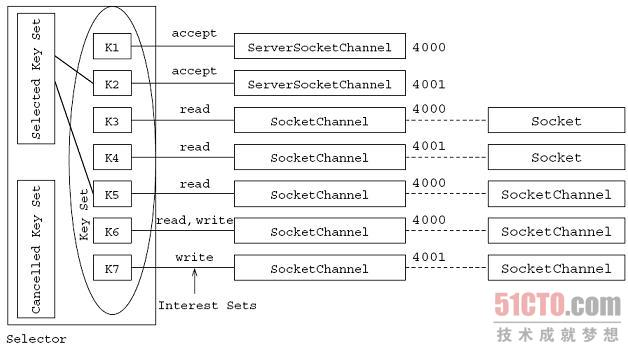
\includegraphics[scale=.6]{img/05.01.jpg}
			\caption{Selector与其关联的键集}
			\label{fig:selector.and.its.key.set}
		\end{figure}

		Selected Key Set: 选择键集; 

		Cancelled Key Set:注销键集; 

		Key Set:键集;

		Interest Sets:兴趣操作集 

	\subsection{选取和识别准备就绪的信道}

		在信道上注册了选择器,并由关联的键指定了感兴趣的I/O操作集后,我们就只需要坐下来等待I/O了。这要使用选择器来完成。

		Selector: 等待信道准备就绪

		\lstinputlisting[language=Java,firstline=301,lastline=304]{src/ch05/TCPEchoClientNonblocking.txt}

	select()方法用于从已经注册的信道中返回在感兴趣的I/O操作集上准备就绪的信道总数。(例如,兴趣操作集中包含\verb|OP_READ|的信道有数据可读,或包含\verb|OP_ACCEPT|的信道有连接请求待接受。)以上三个select方法的惟一区别在于它们的阻塞行为。无参数的select方法会阻塞等待,直到至少有一个注册信道中有感兴趣的操作准备就绪,或有别的线程调用了该选择器的wakeup()方法(这种情况下select方法将返回0)。以超时时长作为参数的select方法也会阻塞等待,直到至少有一个信道准备就绪,或等待时间超过了指定的毫秒数(正数),或者有另一个线程调用其wakeup()方法。selectNow()方法是一个非阻塞版本:它总是立即返回,如果没有信道准备就绪,则返回0。wakeup()方法可以使当前阻塞(也就是说在另一个线程中阻塞)的任何一种select方法立即返回;如果当前没有select方法阻塞,下一次调用这三种方法的任何一个都将立即返回。

	选择之后,我们需要知道哪些信道准备好了特定的I/O操作。每个选择器都维护了一个已选键集(selected-key set),与这些键关联的信道都有即将发生的特定I/O操作。通过调用selectedKeys()方法可以访问已选键集,该方法返回一组SelectionKey。我们可以在这组键上进行迭代,分别处理等待在每个键关联的信道上的I/O操作。

		\lstinputlisting[language=Java,firstline=307,lastline=312]{src/ch05/TCPEchoClientNonblocking.txt}

		图5.1中的选择器的已选键集中有两个键:K2和K5。

		Selector: 获取键集

		\lstinputlisting[language=Java,firstline=315,lastline=316]{src/ch05/TCPEchoClientNonblocking.txt}

		以上方法返回选择器的不同键集。keys()方法返回当前已注册的所有键。返回的键集是不可修改的:任何对其进行直接修改的尝试(如,调用其remove()方法)都将抛出UnsupportedOperationException异常。selectedKeys()方法用于返回上次调用select()方法时,被"选中"的已准备好进行I/O操作的键。重要提示:selectedKeys()方法返回的键集是可修改的,实际上在两次调用select()方法之间,都必须"手工"将其清空。换句话说,select方法只会在已有的所选键集上添加键,它们不会创建新的键集。

		所选键集指示了哪些信道当前可以进行I/O操作。对于选中的每个信道,我们需要知道它们各自准备好的特定I/O操作。除了兴趣操作集外,每个键还维护了一个即将进行的I/O操作集,称为就绪操作集(ready set)。

		SelectionKey: 查找就绪的I/O操作

		\lstinputlisting[language=Java,firstline=319,lastline=324]{src/ch05/TCPEchoClientNonblocking.txt}

		对于给定的键,可以使用readyOps()方法或其他指示方法来确定兴趣集中的哪些I/O操作可以执行。readyOps()方法以位图的形式返回所有准备就绪的操作集。其他方法用于分别检查各种操作是否可用。

		例如,查看键关联的信道上是否有正在等待的读操作,可以使用以下代码:

		\lstinputlisting[language=Java,firstline=328,lastline=328]{src/ch05/TCPEchoClientNonblocking.txt}

		或

		\lstinputlisting[language=Java,firstline=329,lastline=329]{src/ch05/TCPEchoClientNonblocking.txt}

		选择器的已选键集中的键,以及每个键中准备就绪的操作,都是由select()方法来确定的。随着时间的推进,这些信息可能会过时。其他线程可能会处理准备就绪的I/O操作。同时,键也不是永远存在的。当其关联的信道或选择器关闭时,键也将失效。通过调用其cancel()方法可以显示地将键设置为无效。调用其isValid()方法可以检测一个键的有效性。无效的键将添加到选择器的注销键集中,并在下次调用任一种形式的select()方法或close()方法时从键集中移除。(当然,从键集中移除键意味着与它关联的信道也不再受监听。)

	\subsection{信道附件附件}


		当一个信道准备好进行I/O操作时,通常还需要额外的信息来处理请求。例如,在前面的回显协议中,当客户端信道准备好写操作时,就需要有数据可写。当然,我们所需要的可写数据是由之前同一信道上的读操作收集的,但是在其可写之前,这些数据存放在什么地方呢?另一个例子是第3章中的成帧过程。如果一个消息一次传来了多个字节,我们需要保存已接收的部分消息,直到完整个消息接收完成。这两种情况都需要维护每个信道的状态信息。然而,我们非常幸运!SelectionKey通过使用附件使保存每个信道的状态变得容易。

		SelectionKey: 查找准备就绪的I/O操作

		\lstinputlisting[language=Java,firstline=331,lastline=332]{src/ch05/TCPEchoClientNonblocking.txt}

		每个键可以有一个附件,数据类型只能是Object类。附件可以在信道第一次调用register()方法时与之关联,或者后来再使用attach()方法直接添加到键上。通过SelectionKey的attachment()方法可以访问键的附件。 

	\subsection{Selector小结}

		总的来说,使用Selector的步骤如下:

		I.创建一个Selector实例。

		II.将其注册到各种信道,指定每个信道上感兴趣的I/O操作。

		III.重复执行:

		1.调用一种select方法。

		2.获取选取的键列表。

		3.对于已选键集中的每个键,

		a.获取信道,并从键中获取附件(如果合适的话)

		b.确定准备就绪的操作并执行。如果是accept操作,将接受的信道设置为非阻塞模式,并将其与选择器注册。

		c.如果需要,修改键的兴趣操作集

		d.从已选键集中移除键

		如果选择器告诉了你什么时候I/O操作准备就绪,你还需要非阻塞I/O吗?答案是肯定的。信道在已选键集中的键并不能确保非阻塞I/O,因为调用了select()方法后,键集信息可能会过时。另外,阻塞式写操作会阻塞等待直到写完所有的字节,而就绪集中的\verb|OP_WRITE|仅表示至少有一个字节可写。实际上,只有非阻塞模式的信道才能与选择器进行注册:如果信道在阻塞模式,SelectableChannel类的register()方法将抛出IllegalBlockingModeException异常。

\section{数据报(UDP)信道}

	Java的NIO包通过DatagramChannel类实现了数据报(UDP)信道。与我们之前看到的其他形式的SelectableChannel一样,DatagramChannel在DatagramSocket上添加了选择和非阻塞行为,以及基于缓冲区的I/O操作能力。

	DatagramChannel: 创建,连接和关闭

	\lstinputlisting[language=Java,firstline=336,lastline=338]{src/ch05/TCPEchoClientNonblocking.txt}

	需要调用DatagramChannel的open()工厂方法来创建一个DatagramChannel实例,该实例是未绑定的。DatagramChannel只是对基本DatagramSocket的一个包装器(wrapper)。使用其socket()方法可以直接访问内部的DatagramSocket实例。这就允许通过调用基本的DatagramSocket方法进行绑定、设置套接字选项等操作。用完DatagramChannel后,要调用它的close()方法将其关闭。

	只要创建了一个DatagramChannel实例,就可以非常直接地发送和接收数据。

	DatagramChannel: 发送和接收

	\lstinputlisting[language=Java,firstline=341,lastline=342]{src/ch05/TCPEchoClientNonblocking.txt}

	send()方法用于创建一个包含了给定ByteBuffer中的数据的数据报文,并将其发送到目的地址指定的SocketAddress上。receive()方法用于将接收到的数据报文存入指定缓冲区并返回发送者的地址。重要提示:如果缓冲区的剩余空间小于数据报文中的数据大小,多余的数据将毫无提示地丢弃。

	以下代码段用于创建一个DatagramChannel实例,并将UTF-16编码的字符串"Hello"发送到运行在同一主机的5000端口上的UDP服务器上。

	\lstinputlisting[language=Java,firstline=344,lastline=345]{src/ch05/TCPEchoClientNonblocking.txt}

	以下代码段用于创建一个DatagramChannel实例,将底层的套接字绑定到5000端口,接收最长为20字节的数据报文,并将字节转换成使用UTF-16编码的字符串。

	\lstinputlisting[language=Java,firstline=348,lastline=354]{src/ch05/TCPEchoClientNonblocking.txt}

	在上面的send()实例中,调用send()方法时并没有显式地绑定本地端口,因此将随机选择一个可用端口。相应的receive()方法用于返回一个SocketAddress,其中包含了端口号。

	如果总是向同一个远程终端发送或接收数据,我们可以选择调用connect()方法,并使用 SocketAddress指定远程终端的地址。

	DatagramChannel: 连接DatagramChannel

	\lstinputlisting[language=Java,firstline=358,lastline=366]{src/ch05/TCPEchoClientNonblocking.txt}

	这些方法限制我们只能通过指定的地址发送和接收数据。为什么要这样做呢?原因之一是调用connect()方法后,可以使用read()和write()方法来代替receive()和send()方法,并且不需要处理远程地址。read()和write()方法分别用于接收和发送一个数据报文。分散式读操作以一个ByteBuffer数组为参数,只接收一个数据报文,并按顺序将其填入缓冲区中。聚集式写操作将缓冲区数组中的所有字节连接起来创建一个要传输的数据报文。重要提示:现在能够发送的最大数据报文可以包含65507个字节,试图发送更多的数据将被无提示地截断。

	使用connect()方法的另一个好处是,已建立连接的数据报文信道可能只接收从指定终端发送来的数据,因此我们不需要测试接收端的有效性。注意,DatagramChannel的connect()方法只起到限制发送和接收终端的作用,连接时并没有数据包在SocketChannel上进行交换,而且也不需要像SocketChannel那样等待或测试连接是否完成。(见第6章)

	到目前为止DatagramChannel看起来与DatagramSocket非常相似。数据报文信道和套接字的主要区别是,信道可以进行非阻塞I/O操作和使用选择器。DatagramChannel中选择器的创建,信道的注册、选择等,与SocketChannel几乎一模一样。有一个区别是DatagramChannel不能注册连接I/O操作,不过也不需要这样做,因为DatagramChannel的connect()方法永远不会阻塞。

	DatagramChannel: 设置阻塞行为和使用选择器

	\lstinputlisting[language=Java,firstline=371,lastline=377]{src/ch05/TCPEchoClientNonblocking.txt}

	这些方法的功能与SocketChannel和ServerSocketChannel中的相应方法一样。

	下面使用DatagramChannel对第4章中的DatagramSocket UDP回显服务器进行重写。服务器侦听指定的端口,并将接收到的数据报文简单地回发给客户端。重写后的服务器与原来版本的主要区别是它不会在send()和receive()方法上阻塞等待。

	\lstinputlisting[language=Java,firstline=1]{src/ch05/UDPEchoServerSelector.java}
